\documentclass[a4paper,12pt]{article}
\usepackage[a4paper, margin=2.5cm]{geometry}
\usepackage[pdftex]{graphicx}
\usepackage{tikz}
\usepackage{pgfplots}
\usepackage{enumitem}
\usepackage{float}
\usepackage[document]{ragged2e}
\usepackage[utf8]{inputenc}
\usepackage[T1]{fontenc}
\usepackage[spanish,es-tabla]{babel}
\renewcommand{\shorthandsspanish}{}
\usepackage{xurl}
\usepackage{lipsum}
\usepackage{mwe}
\usepackage{multicol}
\usepackage{siunitx}
\usepackage{listings}
\usepackage{circuitikz}
\usepackage{tabularray}

\graphicspath{ {/home/saikkopat/Documents/school/CE/P4/figures/} }

\title{Práctica 4: Divisor de voltaje y de corriente}
\author{González Cárdenas Ángel Aquilez \and Sánchez González Daniel Iván}

\begin{document}

\begin{titlepage}
	\begin{tikzpicture}[overlay, remember picture]
		\path (current page.north east) ++(-0.3,-1.5) node[below left] {
\includegraphics[width=0.35\textwidth]{/home/saikkopat/Documents/LOGOS IPN/EscudoESCOM}};
	\end{tikzpicture}
	\begin{tikzpicture}[overlay, remember picture]
		\path (current page.north west) ++(1.5,-1) node[below right] {
\includegraphics[width=0.2\textwidth]{/home/saikkopat/Documents/LOGOS IPN/logo}};
	\end{tikzpicture}
	\begin{center}
		\vspace{-1.5cm}
		{\LARGE Instituto Politécnico Nacional\par}
		\vspace{.5cm}
		{\LARGE Escuela Superior de Cómputo\par}
		\vspace{.5cm}
		{\Large Laboratorio de Circuitos Eléctricos\par}
		\vspace{2cm}
		{\large Unidad de aprendizaje:}\\{\Large Circuitos Eléctricos\par}
		\vspace{2cm}
		{\scshape\Huge Práctica 4\par}
		{\itshape\Large Divisor de voltaje y de corriente\par}
		\vfill
		\vspace{.7cm}
		{\Large Grupo: 3CV2\par}
		\vspace{.7cm}
		{\Large Integrantes:\\González Cárdenas Ángel Aquilez\\Sánchez González Daniel Iván\par}
		\vspace{1cm}
		{\Large Profesor: Vázquez Ortiz Mijail\par}
		\vspace{1cm}
		{\large Fecha de realización: 17 de abril de 2023\par}
		{\large Fecha de entrega: 24 de abril de 2023\par}
		\vfill
	\end{center}
\end{titlepage} 

\newpage

\tableofcontents

\newpage

\usepgfplotslibrary{units}

\section*{Objetivo}

\textbf{Objetivo}: El alumno identificará al circuito conocido como \textit{circuito divisor de voltaje} en su
forma más simple. Comprenderá el concepto de \textit{circuito divisor de voltaje} y comparará entre los valores calculados con los valores medidos en cada uno de los
elementos asociados en el circuito de la práctica. Comprenderá la utilidad de estos
circuitos tanto en el análisis de redes más complejas como en aplicaciones donde no se
requiera exactitud ni valores altos en el consumo de corriente.\par

\vspace{0.5cm}

El alumno utilizara los siguientes materiales y equipo:

\begin{multicols}{2}
\textbf{Equipo}\\
\begin{itemize}[nosep]
	\item 1 Multímetro digital
	\item 1 Fuente de voltaje variable de corriente directa
\end{itemize}

\columnbreak

\textbf{Material}\\
\begin{itemize}[nosep]
	\item 1 \textit{Protoboard}
	\item 2 Resistencias de \SI{1}{\kohm} a $\frac{1}{2}$ de \si{\watt}
	\item 2 Resistencias de \SI{470}{\ohm} a $\frac{1}{2}$ de \si{\watt}
	\item 2 Resistencias de \SI{560}{\ohm} a $\frac{1}{2}$ de \si{\watt}
	\item 2 Resistencias de \SI{2.2}{\kohm} a $\frac{1}{2}$ de \si{\watt}
	\item 1 Resistencias de \SI{3.3}{\kohm} a $\frac{1}{2}$ de \si{\watt}
	\item 1 Potenciómetro de \SI{10}{\kohm}
	\item 4 puntas banana-caimán
	\item 4 puntas caimán-caimán
	\item Alambres para conexiones
	\item Pinzas de corte
	\item Pinzas de punta
\end{itemize}

\end{multicols}

\section{Introducción teórica}

\subsection{Divisor de voltaje}

Un circuito como el que se exhibe en la Figura 1 recibe el nombre de \textit{circuito divisor de voltaje} debido a que en cada resistor podemos registrar una caída de voltaje que tiene como valor un submúltiplo exacto del valor de la fuente. El factor de multiplicación que define al submúltiplo se obtiene como función de los resistores que forman el circuito, en la siguiente forma:\\


\begin{figure}[h!]
	\centering
	  \begin{circuitikz}[american, voltage dir=RP]
	  		\draw (0,0)
	  		to[battery, l=$V_{s}$, i=$I$] (0,6) -- (3,6)
	  		to[R, l=$R_1$] (3,4)
	  		to[R, l=$R_2$] (3,2)
	  		to[R, l=$R_3$] (3,0) -- (0,0);
		\end{circuitikz}
	\caption{Circuito 1}
\end{figure}


La corriente $I$ en la única malla del circuito puede obtenerse
por Ley de Ohm con la siguiente expresión:\\

\[
	I = \frac{V_s}{R_1 + R_2 + R_3}
\]

Conocida la corriente, se puede encontrar una expresión para el voltaje en cada resistor en valor absoluto:\\

\[
	V_{R1} = R_1  I = R_1 ( \frac{V_s}{R_1 + R_2 + R_3} )
\]
\[
	V_{R1} = ( \frac{R_1}{R_1 + R_2 + R_3} ) V_s
\]


De la misma forma se puede obtener la caída de voltaje en los otros resistores:\\

\[
	V_{R2} = ( \frac{R_2}{R_1 + R_2 + R_3} ) V_s
\]

\[
	V_{R3} = ( \frac{R_3}{R_1 + R_2 + R_3} ) V_s
\]

\vspace{0.5cm}

Con la expresión ya obtenida para la corriente también se pueden deducir las expresiones voltajes nodales, en los nodos $N_1$, $N_2$ y $N_3$, respecto al nodo común o tierra, como se ilustra en la Figura 2:\\

\vspace{0.5cm}

\begin{figure}[h!]
	\centering
	  \begin{circuitikz}[american, voltage dir=RP]
	  \path (3,6.2) node[anchor=east](N1){$N_1$};
	  \path (9,6.2) node[anchor=west](V1){$V_1$};
	  \path (3,4) node[anchor=east](N2){$N_2$};
	  \path (7,4) node[anchor=west](V2){$V_2$};
	  \path (3,2) node[anchor=east](N3){$N_3$};
	  \path (5,2) node[anchor=west](V3){$V_3$};
	  		\draw (0,0)
	  		to[battery, l=$V_{s}$, i=$I$] (0,6.5) -- (3,6.5)
	  		to[R, l=$R_1$] (3,4)
	  		to[R, l=$R_2$] (3,2)
	  		to[R, l=$R_3$] (3,0) -- (0,0);
	  		\draw (3, 6.2) to[short, *-] (9,6.2) [dashed] to[short, -*] [dashed] (9,0);
	  		\draw (3, 4) to[short, *-] (7,4) [dashed] to[short, -*] [dashed] (7,0);
	  		\draw (3, 2) to[short, *-] (5,2) [dashed] to[short, -*] [dashed] (5,0);
	  		\draw (9,0) node[ground](GND){};
  	  		\draw (7,0) node[ground](GND){};
	  		\draw (5,0) node[ground](GND){};
		\end{circuitikz}
	\caption{Circuito 2}
\end{figure}

\vspace{0.5cm}


En la figura 2 se ilustra la forma de medir el voltaje en cada uno de los nodos, respecto del nodo común, nodo cero, ó nodo de referencia.\\

\[
	V_1 = (R_1 + R_2 + R_3) I = V_s
\]

\[
	V_2 = (R_2 + V_3) I =( \frac{R_2 + R_3}{R_1 + R_2 + R_3} ) V_s
\]
\[
	V_3 = ( \frac{R_3}{R_1 + R_2 + R_3} ) V_s
\]

\subsection{Divisor de corriente}
Según \emph{Boylestad, Salas y Rizo}:
\begin{quote}
La conductancia $G$ se definie como $\frac{1}{R}$. La conductancia total de un circuito en paralelo se determina sumando la conductancia de cada rama. La resistencia total $R_t$ es simplemente $\frac{1}{R_t}$.
\end{quote}

Un circuito como el que se exhibe en la Figura 3 recibe el nombre de \textit{divisor de corriente} ya que la corriente total I se divide en cada resistor. De acuerdo a la ley de Ohm tenemos que:\\


\begin{figure}[h!]
	\centering
	  \begin{circuitikz}[american, voltage dir=RP]
	  		\draw (0,0)
	  		to[battery, l=$V_{s}$, i=$I$] (0,3) -- (6,3)
	  		to[R, l=$R_3$, i=$i_3$] (6,0) -- (0,0);
	  		\draw (2,3) to[R, l=$R_1$, i=$i_1$] (2,0);
	  		\draw (4,3) to[R, l=$R_2$, i=$i_2$] (4,0);
		\end{circuitikz}
	\caption{Circuito 3}
\end{figure}


\[
	I = \frac{V}{R} = VG
\]
\[
	I = I_{R1} + I_{R2} + I_{R3}
\]
\[
	I = V(G_1 + G_2 + G_3)
\]

y despejando los voltajes, tenemos:\\

\[
	V = \frac{I}{G_1 + G_2 + G_3}
\]

Sustituyendo para cada corriente de a cuerdo con la ley de Ohm, tenemos:\\

\[
	I_{R1} = V G_1 = \frac{I G_1}{G_1 + G_2 + G_3}
\]
\[
	I_{R2} = V G_2 = \frac{I G_2}{G_1 + G_2 + G_3}
\]
\[
	I_{R3} = V G_3 = \frac{I G_3}{G_1 + G_2 + G_3}
\]

\newpage

\section{Desarrollo}

\subsection{Divisor de voltaje}

Primero, se ajustó la fuente de voltaje a \SI{10}{\volt} y la corriente de la fuente al máximo.\\
Después, y sin energizar el \textit{protoboard}, se construyo el circuito mostrado en la Figura 4.\\
Luego, de forma análoga al circuito 2 de la Figura 2 se realizaron mediciones para $V_{R1}$, $V_{R2}$, $V_{R3}$, $V_1$, $V_2$, $V_3$, y se registraron los resultados en la Tabla 1.\\

\vspace{0.5cm}

\begin{figure}[h!]
	\centering
	  \begin{circuitikz}[american, voltage dir=RP]
	  		\draw (0,0)
	  		to[battery, l=$\SI{10}{\volt}$] (0,6) -- (3,6)
	  		to[R, a=$R_1$, l=$\SI{1}{\kohm}$] (3,4)
	  		to[R, a=$R_2$, l=$\SI{470}{\ohm}$] (3,2)
	  		to[R, a=$R_3$, l=$\SI{560}{\ohm}$] (3,0) -- (0,0);
		\end{circuitikz}
	\caption{Circuito divisor de voltaje}
\end{figure}

\begin{table}[ht!]
\setlength\tabcolsep{3pt}
\begin{center}
\begin{tblr}{|c c c c|}
\hline
		Dato & Valor teórico & Valor medido & Error \Delta\si{\volt}
		\\ [0.5ex]	\hline
 $ V_{R1} $ & \SI{4.92}{\volt} & \SI{4.89}{\volt} & \SI{0.03}{\volt} \\ \hline
 $ V_{R2} $ & \SI{2.31}{\volt} & \SI{2.34}{\volt} & \SI{0.03}{\volt} \\ \hline
 $ V_{R3} $ & \SI{2.75}{\volt} & \SI{2.75}{\volt} & \SI{0.00}{\volt} \\ \hline
 $ V_1$ & \SI{10}{\volt} & \SI{10}{\volt} & \SI{0.00}{\volt} \\ \hline
 $ V_2$ & \SI{5.08}{\volt} & \SI{5.10}{\volt} & \SI{0.02}{\volt} \\ \hline
 $ V_3$ & \SI{2.77}{\volt} & \SI{2.75}{\volt} & \SI{0.02}{\volt} \\ \hline

\end{tblr}
\label{table:1}
\caption{Valores del circuito divisor de voltaje}
\end{center}
\end{table}

Por otra parte, a partir de la Figura 2, suponga $R_1 = \SI{1}{\kohm}$ y $R_2 = \SI{2.2}{\kohm}$, ¿qué valor de $R_3$ es necesario para tener un voltaje $V_3 = \SI{5}{\volt}$ si $V_s = \SI{10}{\volt}$?\\

\vspace{0.5cm}

Para contestar a la pregunta se utilizó un ejemplo similar, haciendo el valor de las resistencia total del circuito igual a \SI{1}{\kohm}, el voltaje se va a dividir entre el número de resistencias y sus diferentes valores, por lo que si tenemos tres resistencias y queremos distribuir sus valores de forma que para la tercer resistencia nos quede la mitad del valor, con \SI{1}{\kohm}, debemos hacer que $R_1 + R_2 = \frac{\SI{1}{\kohm}}{2} = \SI{500}{\ohm}$, por lo tanto, $R_3 = \SI{500}{\ohm}$. Regresando a nuestra pregunta, como $R_1 + R_2 = \SI{3.2}{\kohm}$, entonces $R_3 = \SI{3.2}{\kohm}$ (Véase Figura 7).\\

\vspace{1cm}

Después, se construyo un circuito divisor de voltaje como el de la Figura 2 y se le suministraron \SI{10}{\volt} de donde, para conseguir que $V_2 = \SI{5}{\volt}$ y $V_2 = \SI{3}{\volt}$ se propuso que $R_1 = \SI{1}{\kohm}$, por lo cual, $R_t = \SI{2}{\kohm}$, y los valores para $R_2$ y $R_3$ se encuentran registrados en la Tabla 2 (véase Figura 8).


\begin{table}[ht!]
\setlength\tabcolsep{3pt}
\begin{center}
\begin{tblr}{|c | c c c|}
\hline
		Dato & $R_1$ & $R_2$ & R_3
		\\ [0.6ex]	\hline
\multicolumn{1}{|p{2cm}|}{\centering $V_2 = \SI{5}{V}$ \hline \\ $V_3 = \SI{3}{V}$} & \SI{1}{\kohm} & \SI{400}{\ohm} & \SI{600}{\kohm} \\ \hline


\end{tblr}
\label{table:2}
\caption{Valores medidos del circuito divisor de voltaje}
\end{center}
\end{table}


\subsection{Divisor de corriente}

Primero, se ajustó la fuente de voltaje a \SI{10}{\volt} y la corriente de la fuente al máximo.\\
Después, y sin energizar el \textit{protoboard}, se construyo el circuito mostrado en la Figura 5.\\
Luego, se realizaron las mediciones de corriente para $I_{R1}$, $I_{R2}$, $I_{R3}$, $I_{R4}$. Los resultados se registraron en la Tabla 3.


\begin{figure}[h!]
	\centering
	  \begin{circuitikz}[american, voltage dir=RP]
	  		\draw (0,0)
	  		to[battery, l=$\SI{10}{\volt}$, i=$I$] (0,6) -- (3,6)
			to[R, a=$R_1$, l=$\SI{1}{\kohm}$] (3,3) -- (9,3)
			to[R, a=$R_4$, l=$\SI{3.3}{\kohm}$, i=$I_{R4}$] (9,0) -- (0,0);
	  		\draw (3,3) to[R, a=$R_2$,l=$\SI{1}{\kohm}$, i=$I_{R2}$] (3,0);
	  		\draw (6,3) to[R, a=$R_3$,l=$\SI{2.2}{\kohm}$, i=$I_{R3}$] (6,0);
	  		
		\end{circuitikz}
	\caption{Circuito divisor de corriente}
\end{figure}


\begin{table}[ht!]
\setlength\tabcolsep{3pt}
\begin{center}
\begin{tblr}{|c c c c|}
\hline
		Dato & Valor teórico & Valor medido & Error \Delta\si{\A}
		\\ [0.5ex]	\hline
 $ I_{R1} $ & \SI{6.37}{\mA} & \SI{6.351}{\mA} & \SI{0.021}{\mA} \\ \hline
 $ I_{R2} $ & \SI{3.624}{\mA} & \SI{3.626}{\mA} & \SI{0.002}{\mA} \\ \hline
 $ I_{R3} $ & \SI{1.64}{\mA} & \SI{1.620}{\mA} & \SI{0.02}{\mA} \\ \hline
 $ I_{R4} $ & \SI{1.09}{\mA} & \SI{1.123}{\mA} & \SI{0.021}{\mA} \\ \hline
 $ I_{total}$ & \SI{6.37}{\mA} & \SI{6.351}{\mA} & \SI{0.021}{\mA} \\ \hline

\end{tblr}
\label{table:3}
\caption{Valores del circuito divisor de corriente}
\end{center}
\end{table}


\newpage

\section{Cuestionario}

\vspace{1cm}

\begin{enumerate}

\item ¿A qué se debe la existencia del error o desviación del valor medido respecto del valor calculado?\\
Se debe a la variación del valor real de cada elemento resistivo respecto a su valor indicado por su código de colores y la tolerancia que se indica, lo cual impacta los valores medidos de corriente y voltaje además de un valor adicional muy pequeño de la resistencia en el cableado utilizado para medir los valores.

\item ¿Cuál es la utilidad del \textit{divisor de voltaje} para el análisis de circuitos eléctricos?\\
Nos permite calcular las diferentes caídas de voltaje a través de un circuito en serie sin realizar un circuito equivalente.

\item ¿Cuál es la utilidad del \textit{divisor de corriente} para el análisis de circuitos eléctricos?\\
Nos permite calcular como se distribuye de la corriente a través de los diferentes elementos resistivos en un circuito en paralelo.

\item ¿Puede extenderse los circuitos divisores de  voltaje y de corriente a un número mayor de resistores?\\
Sí, ya que puede reducirse a un circuito equivalente o bien, deducir una regla de divisor de corriente o voltaje a partir de la Ley de Ohm.

\item Si los voltajes en cada nodo fueran requeridos con valores específicos predeterminados, ¿qué debería hacerse para obtener dichos valores?\\
De manera análoga a lo registrado en el desarrollo, debe proponerse un valor de resistencia total para el circuito y a partir del número de elementos necesarios en el circuito, calcular con base en el porcentaje que cada resistencia \emph{consumirá}, o bien, determinar las diferentes caídas de voltaje.

\end{enumerate}

\newpage

\section{Conclusiones}

\vspace{.5cm}

{\Large González Cárdenas Ángel Aquilez}\\
\vspace{.3cm}
Al concluir la práctica, se aplicó la regla del divisor de voltaje en la primer parte del desarrollo, donde se comprobaron las caídas de voltaje a lo largo de un circuito resistivo en serie y se logró determinar un voltaje especifico a partir de un valor resistivo dado o propuesto. Luego, de comprobó la regla del divisor de corriente al contrastar los diferentes valores medidos de corriente para cada rama del circuito.\par

\vspace{1cm}

{\Large Sánchez González Daniel Iván}\\
\vspace{.3cm}
En la primer parte del desarrollo de la práctica, se comprobó la regla del divisor de voltaje, así como se determinó un valor de voltaje para un determinado nodo a partir de un valor resistivo preestablecido y para una configuración totalmente arbitraria a partir de porcentajes respecto a la resistencia total y el valor del voltaje suministrado al circuito.
En la segunda parte, se comprobó la regla del divisor de corriente y se contrastaron los cálculos realizados con las mediciones.\par

\section{Bibliografía}

\begin{itemize}
\item Boylestad, R. L., Salas, R. N., y Rizo, J. F. P. (2011). Introducción al análsis de circuitos. (página 451).
\end{itemize}

\section{Anexos}
\subsection{Simulaciones de los circuitos}

A continuación de presentan los resultados de las simulaciones de los circuitos de las figuras 4 y 5, y los ejercicios propuestos para la sección 2.1, para contrastarlos con las mediciones y cálculos realizados. Se generaron gracias a la aplicación multiplataforma \textit{EveryCircuit}\texttrademark. \\




\begin{figure}[!h]
\centering
	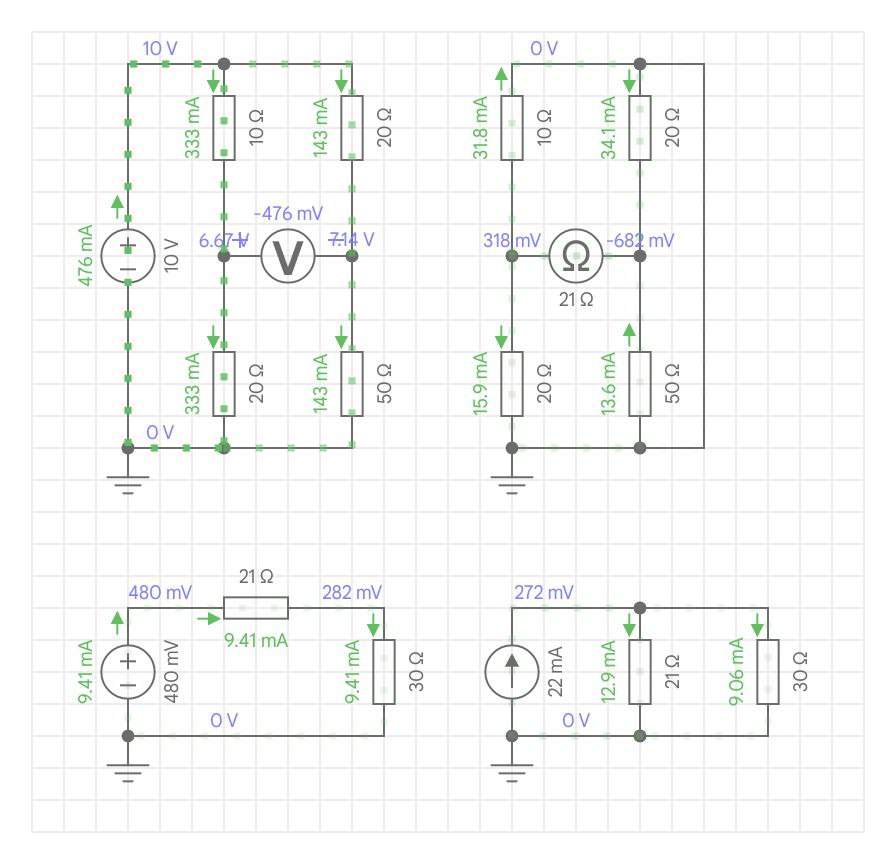
\includegraphics[width=.8\textwidth]{fig1}
	\label{fig6}
	 \caption{Simulación del circuito de la Figura 4}
\end{figure}



\begin{figure}[!h]
\centering
	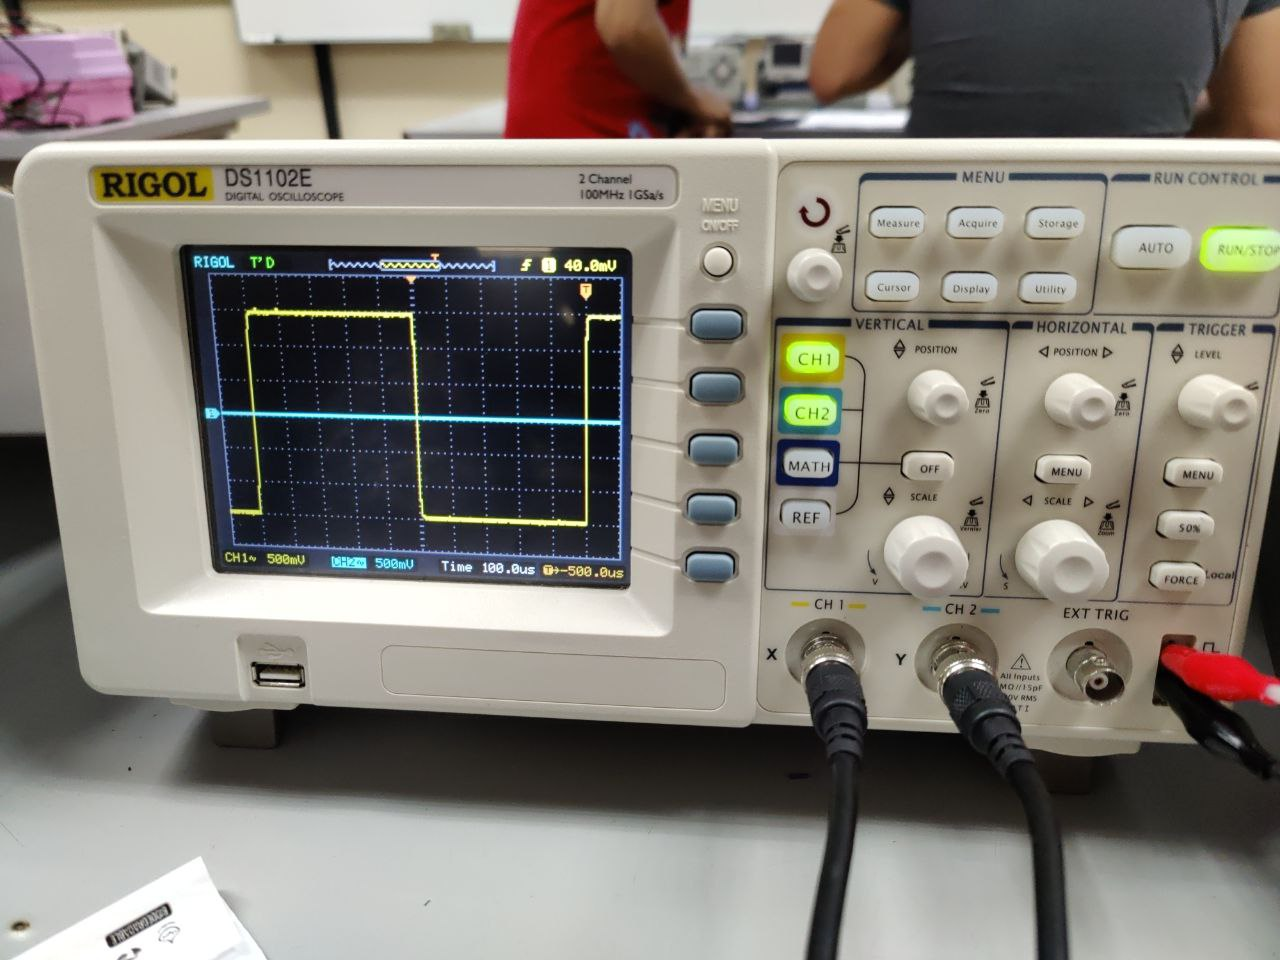
\includegraphics[width=.8\textwidth]{fig2}
	\label{fig7}
	\caption{Circuito divisor de voltaje}
\end{figure}


\begin{figure}[!h]
\centering
	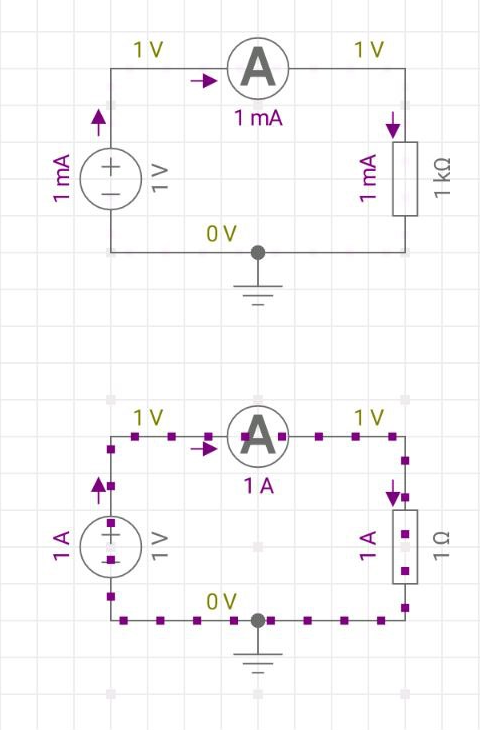
\includegraphics[width=.8\textwidth]{fig3}
	\label{fig8}
	\caption{Circuito divisor de voltaje}
\end{figure}


\begin{figure}[!h]
\centering
	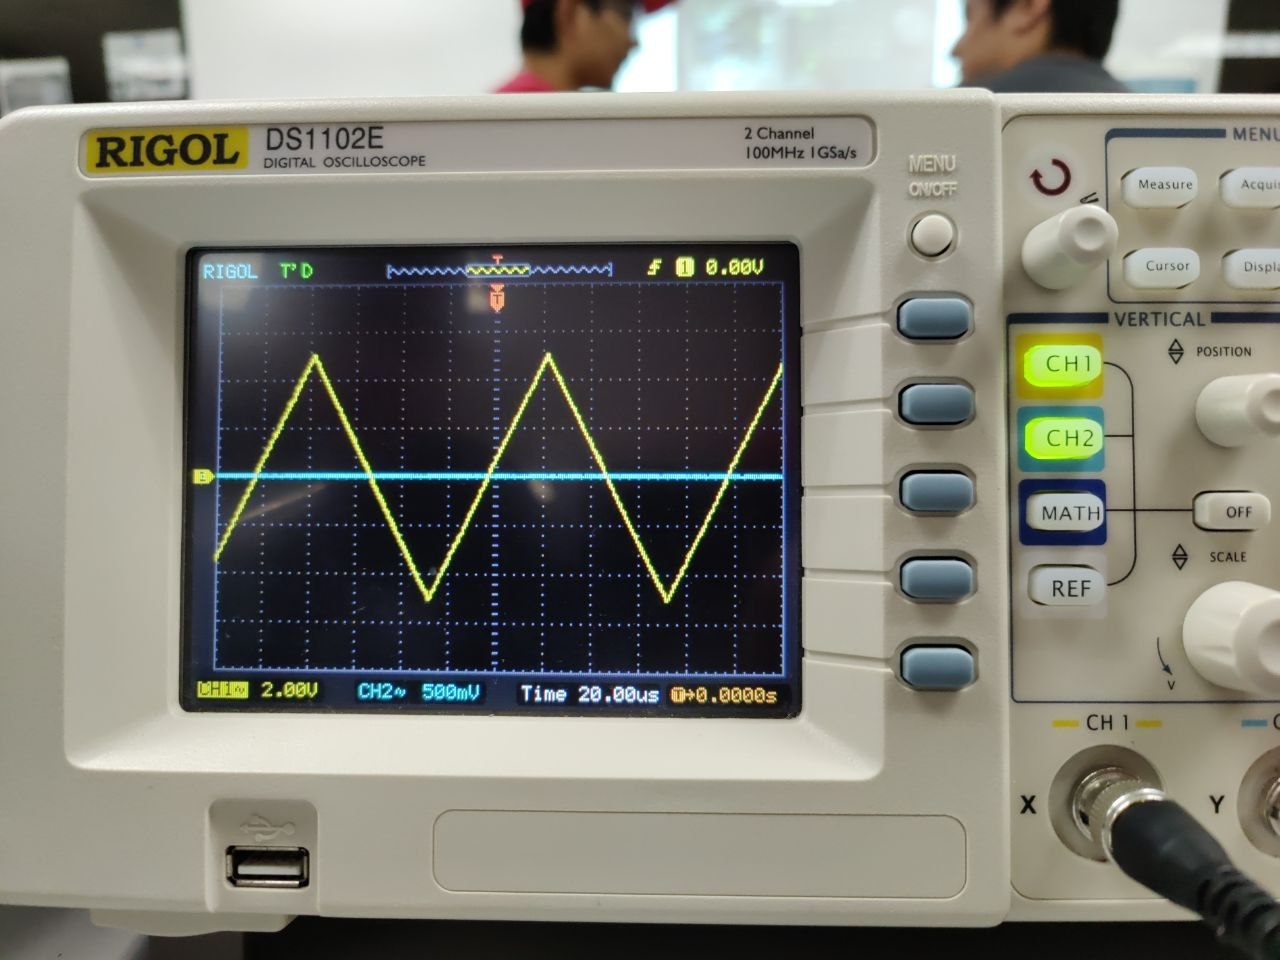
\includegraphics[width=.8\textwidth]{fig4}
	\label{fig9}
	 \caption{Simulación del circuito de la Figura 5}
\end{figure}


\end{document}